\documentclass[11pt,a4paper]{article}
\usepackage[a4paper,margin=22mm,headheight=15pt]{geometry}
\usepackage[T1]{fontenc}
\usepackage[utf8]{inputenc}
\usepackage{lmodern}
\usepackage{microtype}
\usepackage{xcolor}
\usepackage{amsmath,amssymb,mathtools}
\usepackage{booktabs,longtable,array,tabularx}
\usepackage{enumitem}
\usepackage{fancyhdr}
\usepackage{hyperref}
\usepackage{tikz}
\usetikzlibrary{arrows.meta,positioning,shapes.geometric,shapes.misc,fit,calc,decorations.pathreplacing,patterns}
\usepackage{pgfplots}
\pgfplotsset{compat=1.18}
\usepackage[most]{tcolorbox}
\usepackage{listings}
\definecolor{navy}{HTML}{183153}
\definecolor{teal}{HTML}{137C8B}
\definecolor{pale}{HTML}{EEF5F7}
\definecolor{orange}{HTML}{C56A20}
\definecolor{rednote}{HTML}{A83232}
\definecolor{greenformula}{HTML}{237A57}
\hypersetup{colorlinks=true,linkcolor=navy,urlcolor=teal,citecolor=teal,pdftitle={Study Notes},pdfauthor={Compiled from Notion study notes}}
\pagestyle{fancy}\fancyhf{}\lhead{\small IIT Madras BS -- Study Notes}\rhead{\small\nouppercase{\leftmark}}\cfoot{\thepage}
\setlength{\parindent}{0pt}\setlength{\parskip}{5pt}
\setlist[itemize]{leftmargin=1.4em,itemsep=2pt,topsep=3pt}
\setlist[enumerate]{leftmargin=1.7em,itemsep=2pt,topsep=3pt}
\newtcolorbox{conceptbox}{colback=pale,colframe=teal!70!black,title=Concept,breakable,fonttitle=\bfseries}
\newtcolorbox{formulaBox}{colback=greenformula!5,colframe=greenformula,title=Core formula,breakable,fonttitle=\bfseries}
\newtcolorbox{exampleBox}{colback=orange!6,colframe=orange,title=Worked example,breakable,fonttitle=\bfseries}
\newtcolorbox{warningBox}{colback=rednote!5,colframe=rednote,title=Common trap,breakable,fonttitle=\bfseries}
\lstset{basicstyle=\ttfamily\small,keywordstyle=\color{navy}\bfseries,commentstyle=\color{teal!70!black},stringstyle=\color{orange!90!black},numbers=left,numberstyle=\tiny\color{gray},numbersep=8pt,frame=single,rulecolor=\color{black!20},breaklines=true,showstringspaces=false,tabsize=4}
\newcommand{\topicflow}[1]{\begin{center}\begin{tikzpicture}[node distance=5mm,>=Latex,every node/.style={draw=teal!70!black,rounded corners,fill=pale,align=center,text width=0.79\linewidth,minimum height=7mm,font=\small}, every path/.style={->,thick,draw=teal}] #1 \end{tikzpicture}\end{center}}
\begin{document}
\begin{titlepage}
\centering\vspace*{20mm}
{\Large\color{teal} IIT MADRAS BS DEGREE PROGRAMME\par}\vspace{12mm}
{\Huge\bfseries\color{navy} Introduction to C Programming\par}\vspace{5mm}
{\Large Language fundamentals, memory, pointers, strings, allocation, files and debugging\par}\vspace{15mm}
\begin{tcolorbox}[width=0.88\textwidth,colback=pale,colframe=teal]
Converted from the corresponding Notion study guide. This editable LaTeX source includes typeset equations, tables, recreated TikZ flowcharts, and PGFPlots graphs. The notes are syllabus-aligned study material, not a verbatim transcript of every lecture.
\end{tcolorbox}
\vfill
\href{https://app.notion.com/p/403a8fc810f681228557d063ea987071}{Open original Notion study notes}\par
\vspace{5mm}{\large Compiled 29 October 2026\par}
\end{titlepage}
\tableofcontents\clearpage

\section{Course overview and computer model}
C is a compiled, procedural systems language. This guide follows the course progression from program basics and number representation to expressions, control flow, functions, pointers, arrays and strings, structures, dynamic memory, files, bit operations, and multi-file projects.
\topicflow{\node (a) {Source code};\node (b) [below=of a] {Preprocessing};\node (c) [below=of b] {Compilation};\node (d) [below=of c] {Assembly};\node (e) [below=of d] {Linking};\node (f) [below=of e] {Executable};\draw (a)--(b);\draw (b)--(c);\draw (c)--(d);\draw (d)--(e);\draw (e)--(f);}
\section{Memory and the first program}
A program transforms input/state into output. A simplified process memory view contains code, global/static objects, a stack commonly used for automatic objects and calls, and a heap used for dynamic allocation. Exact layout is operating-system and implementation dependent.
\begin{center}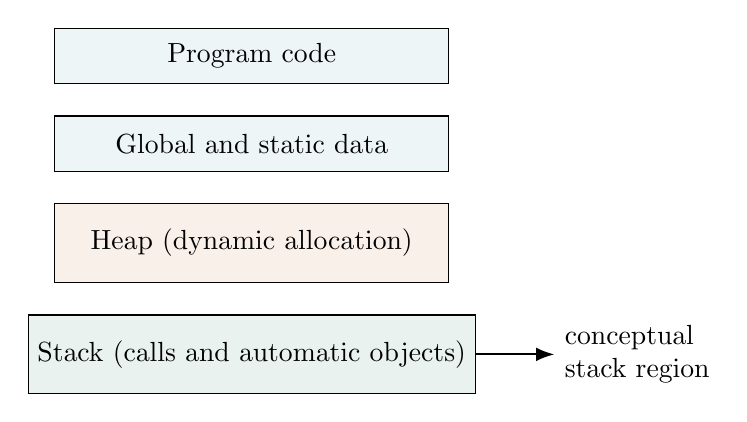
\begin{tikzpicture}[node distance=4mm,>=Latex]\node[draw,fill=pale,minimum width=5cm,minimum height=7mm] (code) {Program code};\node[draw,fill=pale,minimum width=5cm,minimum height=7mm,below=of code] (data) {Global and static data};\node[draw,fill=orange!10,minimum width=5cm,minimum height=10mm,below=of data] (heap) {Heap (dynamic allocation)};\node[draw,fill=greenformula!10,minimum width=5cm,minimum height=10mm,below=of heap] (stack) {Stack (calls and automatic objects)};\draw[->,thick] (stack.east) -- ++(1,0) node[right,align=left]{conceptual\\stack region};\end{tikzpicture}\end{center}
A minimal program:
\begin{lstlisting}[language=C]
#include <stdio.h>

int main(void) {
    printf("Hello, world!\n");
    return 0;
}
\end{lstlisting}
\section{Binary, hexadecimal, types and expressions}
An unsigned binary value is a weighted sum $\sum_{i=0}^{n-1}b_i2^i$. One hexadecimal digit represents four bits. For example, $101101_2=32+8+4+1=45_{10}=2D_{16}$. Two's complement with $n$ bits represents signed values from $-2^{n-1}$ to $2^{n-1}-1$.
C types control value representation and operations. Integer division truncates toward zero; floating-point division retains fractional values if an operand is floating-point. Integer overflow, conversions, and signedness require careful analysis.
\begin{exampleBox}\texttt{7 / 2} evaluates to integer $3$, while \texttt{7.0 / 2} evaluates to $3.5$.
\end{exampleBox}
\section{Branches and loops}
\texttt{if}/\texttt{else} selects a branch; \texttt{switch} selects among cases; loops repeat a block. A counted loop typically has initialisation, condition, body, and update. Check boundary conditions to avoid off-by-one errors.
\begin{lstlisting}[language=C]
int total = 0;
for (int i = 1; i <= 4; ++i) {
    total += i;
}
printf("%d\n", total); /* prints 10 */
\end{lstlisting}
\begin{center}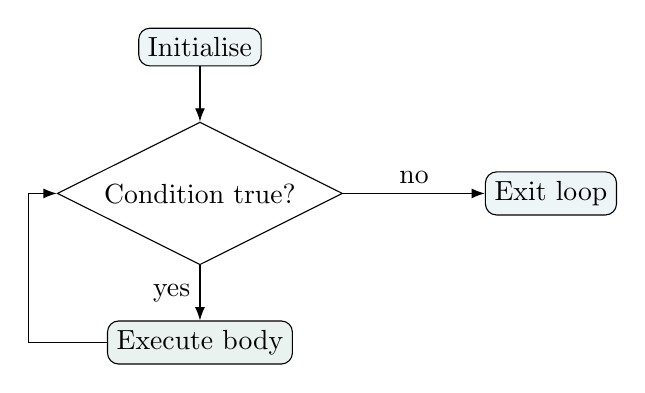
\begin{tikzpicture}[node distance=7mm,>=Latex]\node[draw,rounded corners,fill=pale] (start) {Initialise};\node[draw,diamond,aspect=2,below=of start] (cond) {Condition true?};\node[draw,rounded corners,fill=greenformula!10,below=of cond] (body) {Execute body};\node[draw,rounded corners,fill=pale,right=18mm of cond] (end) {Exit loop};\draw[->] (start)--(cond);\draw[->] (cond)--node[left]{yes}(body);\draw[->] (body.west) -- ++(-1,0) |- (cond.west);\draw[->] (cond)--node[above]{no}(end);\end{tikzpicture}\end{center}
\section{Functions, scope and recursion}
A function declaration (prototype) states the interface; its definition supplies the body. C passes arguments by value. To let a function modify a caller's object, pass a pointer to it. Scope determines where an identifier is visible; lifetime determines how long the object exists. Recursion requires a base case and progress toward it.
\begin{lstlisting}[language=C]
int square(int x); /* prototype */

int square(int x) {
    return x * x;
}
\end{lstlisting}
\section{Pointers and arrays}
A pointer stores an address of an object or function of a compatible type. \texttt{\&x} obtains an object's address; \texttt{*p} accesses the pointed-to object. Pointer arithmetic is constrained by array object boundaries. A pointer must be valid before dereferencing.
\begin{lstlisting}[language=C]
int n = 5;
int *p = &n;
*p += 3;
printf("%d\n", n); /* prints 8 */
\end{lstlisting}
\begin{center}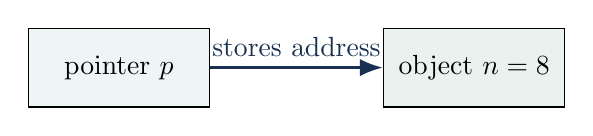
\begin{tikzpicture}[>=Latex,node distance=7mm]\node[draw,fill=pale,minimum width=23mm,minimum height=10mm] (p) {pointer $p$};\node[draw,fill=greenformula!10,minimum width=23mm,minimum height=10mm,right=22mm of p] (n) {object $n=8$};\draw[->,very thick,navy] (p.east)--node[above]{stores address}(n.west);\end{tikzpicture}\end{center}
An array contains contiguous elements indexed from zero. For \texttt{int a[3] = \{4, 5, 6\};}, the valid indices are 0, 1 and 2; \texttt{a[3]} is out of bounds. The size of an array is not the same as the size of a pointer.
\begin{center}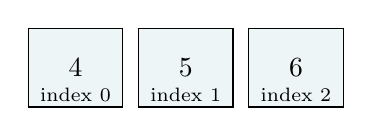
\begin{tikzpicture}[>=Latex]\foreach \i/\v in {0/4,1/5,2/6}{\node[draw,minimum width=12mm,minimum height=10mm,fill=pale] at (\i*1.4,0) {\v};\node at (\i*1.4,-.35) {\scriptsize index \i};}\end{tikzpicture}\end{center}
\section{Strings}
A C string is a sequence of characters terminated by the null character \texttt{'\\0'}. The literal \texttt{"cat"} has four array elements when stored as \texttt{char s[]}: three letters and the terminator. \texttt{sizeof s} is 4 in that context; \texttt{strlen(s)} is 3.
\begin{lstlisting}[language=C]
char s[] = "cat";
/* c  a  t  \0 */
if (strcmp(s, "cat") == 0) {
    puts("match");
}
\end{lstlisting}
Use \texttt{strcmp} to compare string contents, not \texttt{==} (which compares pointer values in common expression contexts). Avoid buffer overflows; validate lengths and prefer bounded input approaches such as \texttt{fgets}.
\section{Structures, unions, enumerations and typedef}
A \texttt{struct} groups fields which can all be present at once. A \texttt{union} overlays alternative members in shared storage. An \texttt{enum} defines named integer constants. \texttt{typedef} introduces an alias for a type. Use the arrow operator \texttt{->} to access a field through a pointer to a structure.
\begin{lstlisting}[language=C]
typedef struct {
    unsigned id;
    double value;
} Reading;

Reading r = {.id = 1, .value = 2.5};
Reading *ptr = &r;
printf("%.1f\n", ptr->value);
\end{lstlisting}
\section{Dynamic memory}
\texttt{malloc} allocates uninitialised storage; \texttt{calloc} allocates and zero-initialises bytes; \texttt{realloc} attempts to resize an allocation; \texttt{free} releases it. Check allocation results and arithmetic used to calculate size. After freeing, do not dereference the old pointer; avoid double-free and use-after-free.
\begin{lstlisting}[language=C]
size_t count = 10;
int *values = malloc(count * sizeof *values);
if (values == NULL) {
    /* handle allocation failure */
    return 1;
}
/* Initialise values before reading them. */
free(values);
values = NULL;
\end{lstlisting}
\begin{center}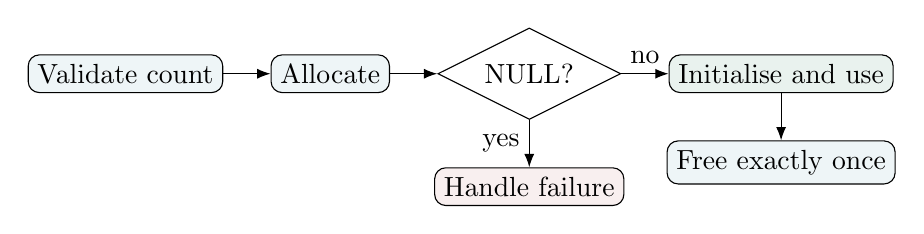
\begin{tikzpicture}[node distance=6mm,>=Latex]\node[draw,rounded corners,fill=pale] (req) {Validate count};\node[draw,rounded corners,fill=pale,right=of req] (alloc) {Allocate};\node[draw,diamond,aspect=2,right=of alloc] (ok) {NULL?};\node[draw,rounded corners,fill=rednote!8,below=of ok] (fail) {Handle failure};\node[draw,rounded corners,fill=greenformula!10,right=of ok] (use) {Initialise and use};\node[draw,rounded corners,fill=pale,below=of use] (free) {Free exactly once};\draw[->] (req)--(alloc);\draw[->] (alloc)--(ok);\draw[->] (ok)--node[left]{yes}(fail);\draw[->] (ok)--node[above]{no}(use);\draw[->] (use)--(free);\end{tikzpicture}\end{center}
\section{File I/O and multi-file programs}
Typical file workflow: open, check the returned pointer, read/write, check operation results, and close. Use \texttt{fgets} for line-based input. Organise declarations in headers and definitions in source files; header guards prevent repeated inclusion. Link all required translation units.
\begin{lstlisting}[language=C]
FILE *fp = fopen("data.txt", "r");
if (fp == NULL) {
    perror("data.txt");
    return 1;
}
char buffer[256];
while (fgets(buffer, sizeof buffer, fp) != NULL) {
    fputs(buffer, stdout);
}
if (ferror(fp)) {
    /* handle read failure */
}
fclose(fp);
\end{lstlisting}
\section{Bitwise operations and masks}
Bitwise AND, OR, XOR, NOT, left shift and right shift operate on integer representations. A mask selects bits for setting, clearing or toggling. Use unsigned types for bit-manipulation patterns where appropriate and be careful with shift widths and signed shifts.
\begin{lstlisting}[language=C]
unsigned flags = 0u;
unsigned mask = 1u << 3;
flags |= mask;    /* set bit 3 */
flags &= ~mask;   /* clear bit 3 */
flags ^= mask;    /* toggle bit 3 */
\end{lstlisting}
\section{Common defects}
\begin{warningBox}
Uninitialised reads; out-of-bounds access; invalid, null or dangling pointer dereference; use-after-free; double-free; returning a pointer to a local automatic object; incorrect format specifiers; unchecked allocation or file errors; unsafe input; integer overflow; data races in concurrent code; and reliance on undefined behaviour.
\end{warningBox}
Debug by reproducing with a minimal case, reading the first meaningful compiler warning, checking initialisation and bounds, verifying pointer lifetime/ownership, inspecting return codes, and rerunning regression tests after fixes. Enable warnings and use sanitizers/debuggers when available.
\section{Practice and quick reference}
\begin{longtable}{p{0.32\linewidth}p{0.6\linewidth}}\toprule
Task & Safe pattern \\ \midrule
Print an integer & \lstinline|printf("%d\\n", n);| \\
Check integer input & \lstinline|scanf("%d", &n) == 1| \\
Counted loop & \texttt{for (size\_t i=0; i<n; ++i)} \\
Address / dereference & \texttt{\&object} / \texttt{*ptr} \\
String comparison & \texttt{strcmp(a,b) == 0} \\
Allocate & \texttt{malloc(count * sizeof *ptr)} after size checks \\
Read line & \texttt{fgets(buffer, sizeof buffer, fp)} \\
Compile multiple files & \texttt{gcc main.c helper.c -o app} \\
\bottomrule\end{longtable}
\section{Revision checklist}
\begin{itemize}
\item Explain preprocessing, compilation, assembly, linking and runtime.
\item Convert binary, decimal and hexadecimal; reason about signed representations.
\item Trace expressions, branches, loops, function calls and recursion.
\item Draw pointer and array memory layouts; respect object lifetime and bounds.
\item Manage strings with sufficient storage for the null terminator.
\item Use structures, dynamic memory and file I/O with failure checks.
\item Understand bit masks, multi-file builds, compiler warnings and debugging.
\end{itemize}
\section{Source and scope}
Source: \href{https://app.notion.com/p/403a8fc810f681228557d063ea987071}{Introduction to C Programming -- Complete Study Notes and Visual Revision Guide}. Official outlines: \url{https://study.iitm.ac.in/ae/course_pages/BSCS1101.html} and \url{https://study.iitm.ac.in/es/course_pages/CS1101.html}. The code is illustrative and should be compiled under the target compiler/C standard; language details and behaviour may vary by implementation where the standard permits it.
\end{document}
